\chapter{Theoretical Principles}
\label{THEO}
The following chapter describes the necessary theoretical knowledge to understand the research process and development. Close attention is paid to DSLs in general and the difference between internal and external DSLs. Furthermore, the programming language Scala is analysed and is viewed from the DSL implementation perspective. With an introduction to Scala.js, the possibilities and limits of the Scala-to-JavaScript code compiler are illustrated. To provide a better comprehension of the design and development decisions, the MIDI system is introduced and discussed.

\section{Domain Specific Languages}
\label{THEO_DSL}
Almost all programming languages are defined as a Turing complete and a general-purpose language (GPL). However, most programming languages are also designed for a specific purpose. For example, the Java design goal is to develop "highly robust applications on multiple platforms in heterogeneous, distributed networks".\cite{Gosling1996} The Prolog language is associated with artificial intelligence.\cite{Bowen1981} PHP is described as a language which is designed for "web development".\cite{ThePHPGroup} However, these design goals indicate that these languages are more domain-specific than general-purpose languages.\cite{Mernik2005} It is evident that something is more comfortable to use when the instrument is developed for a specific context. For example, PHP opens web development to a larger group of developers as Prolog (despite the opportunity to build web applications in Prolog), since the PHP language and its syntax are closer to this domain—the web-development domain. This is the exact starting point for DSLs—abstract a specific domain problem and make it accessible for the domain experts.

Apart from the fact that any GPL is in a particular way a DSL, in almost all cases a DSL is provided through a GPL. The consequence of this principle is that the DSL has to be implemented with the GPL and has to extend it, to provide a user-friendly language on top.\cite{Ghosh2010} Ghosh and other authors define this concept as "metalinguistic abstraction"\cite[p. 15]{Ghosh2010}. The next two subsections describe two ways to implement a DSL through a GPL, the internal and the external.

\subsection{Internal DSL}
\label{THEO_DSL_INTERN}
Internal (also called embedded) DSLs are often described with, or compared to an application programming interface (API).\cite{Mernik2005, Ghosh2010, Riti2018} Since an internal DSL is a direct subset of the GPL, the syntax must be the same as the GPL. Despite this condition, an internal DSL is well suitable to create a \textit{fluent interface}. The terminology "fluent" is described by Fowler.\cite{Fowler2010} The term means that the DSL is closely developed to the natural language and offers a syntax where the expressions and statements of the DSL are readable like human language. Underneath, the DSL is a concatenation of function calls. In section \ref{THEO_SCALA} the Scala GPL is introduced and it is discussed why the Scala language is a perfect fit for defining internal DSLs.

In the following example, a pseudo-GPL is illustrated. The pseudo-GPL is defined as function calls which are invoked by using \texttt{->}. Consider the domain in which the DSL is applied for: the administration of a shopping market. The domain administrator wants to be able to set product prices and order new products. The traditional GPL approach is to define objects and functions with parameters and take advantage of method chaining.

\begin{center}
\texttt{new Product('coffee')->makeOffer(10)->until(2018-05-14)}
\end{center}

The pseudo code above creates a new object of the type \texttt{product} with the name \texttt{coffee} and calls the class method \texttt{makeOffer} with the price \texttt{10} as argument. Through method chaining a new object of the type \texttt{offer} is returned which provides the function \texttt{until} to set an end date for the offer. This syntax is familiar to developers and programmers. In the next step, the GPL specific elements, like the arrow \texttt{->} and parentheses are highlighted and subsequently eliminated.

\begin{center}
\texttt{ \textbf{new} Product\textbf{('}coffee\textbf{')->}createOffer\textbf{(}10\textbf{)->}until\textbf{(}2018-05-14\textbf{)}}
\end{center}

\begin{center}
\texttt{Product coffee createOffer 10 until 2018-05-14}
\end{center}

An almost fluent sentence was created which is close to the natural language. The next listing will add additional words to complete the statement to an approximately natural sentence.

\begin{center}
\texttt{for the product coffee create an offer of 10 EUR until 2018-05-14}
\end{center}

As in the listings above illustrated, it is possible to create a fluent API just with tools of the GPL. Furthermore, internal DSLs can be classified according to their relation to the host GPL.

\begin{figure}[h]
\caption{GPL Extension and Reduction.\cite{Fleming2015}}
\label{IMG_DSL-RED-EXT}
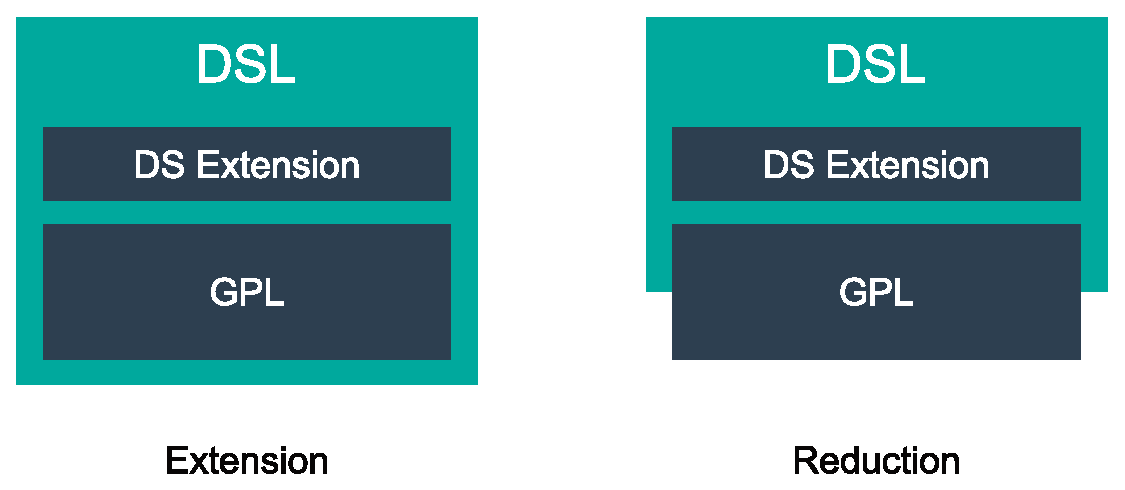
\includegraphics[scale=0.5]{dsl_extension_reduction}
\end{figure}

Figure \ref{IMG_DSL-RED-EXT} shows two classes of internal DSLs. The left side presents the GPL extension. This means that the developer provides the DSL user with the entire GPL functionality and on top of it—the DSL functionality. The right site represents the reduction of the GPL. The advantage of this approach is that the DSL is just an extract of the GPL and reduces its complexity, which, in turn, significantly increases simplicity.\cite{Schmitt2014}

\subsection{External DSL}
\label{THEO_DSL_EXTERN}
In comparison to the internal approach, an external DSL has no restrictions in defining the language since it is completely decoupled from the GPL. Therefore, the developed language can be very close to the language which is used in the target domain. However, the negative aspect of this total flexibility is the effort required in its implementation. Due to the fact that external DSLs are not coupled to the GPL syntax, the parser and interpreter have to be developed additionally. External DSLs are further discussed in chapter \ref{IMPL_SCALALA}.


\section{Scala}
\label{THEO_SCALA}
Scala offers useful tools, to define and develop DSLs. This is because of the circumstance that Scala combines two programming paradigms: object orientated and functional programming. Beyond that, the Scala GPL offers support for function calls without the dot notation or parentheses. The example given in section \ref{THEO_DSL_INTERN} is therefore already valid Scala code. This enables a clean code solution that is also simple to maintain.\cite{Riti2018} Chapter \ref{IMPL_SCALALA} presents essential concepts of Scala. For example: traits, pattern matching, case classes and higher-order functions and why these are necessary and useful for developing DSLs.

\section{Scala.js}
\label{THEO_SCALAJS}
To embrace the developed DSL in a holistic approach, a web-interface was developed. The whole client-application is written in Scala.js. Scala.js is a compiler that translates Scala code to equivalent JavaScript code; like its counterpart TypeScript. It offers an easy to use approach to write familiar Scala code with all its benefits like type safety, immutability, collections and pattern matching. See listings \ref{LS_NATIVE_JS} and \ref{LS_SCALAJS} to compare native JavaScript classes with Scala.js classes.\cite{ScJsDoc}

\begin{lstlisting}[caption={Native JavaScript Class Example}, label=LS_NATIVE_JS]
var Person = function(firstName, lastName) {
  this.firstName = firstName;
  this.lastName = lastName;
};

Person.prototype.fullName = function() {
  return this.firstName + " " + this.lastName;
};
\end{lstlisting}


\begin{lstlisting}[caption={Scala.js Class Example}, label=LS_SCALAJS]
class Person(val firstName: String, val lastName: String) {
  def fullName(): String =
    s"$firstName $lastName"
}
\end{lstlisting}

Furthermore, the compiler provides the possibility to compile any Scala.js source into one stand-alone JavaScript file. Later on, this is an important advantage in the matter of performance. Scala.js is also interoperable with writing type-safe libraries and existing JavaScript libraries. In this study, Scala.js has a central role, since the approach is to teach programming through music within a web environment. It provides and deals with the playback of the written music and handles the communication with the server.


\section{MIDI}
\label{THEO_MIDI}
In this section, the Musical Instrument Digital Interface (MIDI) is explained. Since MIDI is also related to several hardware specifications and a definition of all components is beyond the scope of this study, only the to this thesis relevant aspects are discussed. Originally, MIDI was developed as a communication protocol to control synthesisers by triggering events from a hardware keyboard.\cite{Manning2013} The digital interface and the protocol were standardised in 1982, and the MIDI specification was released in 1983.\cite{MIDIManufacturersAssociation} The MIDI file, and the protocol respectively are based on control sequences and contain no sound files. Hence, MIDI files are typically compact in file size and suitable for transmission between instruments and devices. The file size is one of the properties why the MIDI specification was chosen for this project. Another reason is that the messages (bytes transposed in natural language) are well suited in the context of this study. The messages are divided into control messages and data messages. For example, one data sequence is divided into 3-byte-data sets (simplified representation):

\begin{itemize}
\item\texttt{0x90 NOTE ON} 
\item\texttt{0x3C MIDDLE C} 
\item\texttt{0x40 VELOCITY > 0} 
\end{itemize}

This segmentation allows for a suitable abstraction an easy to create application layer. Java already has the \texttt{javax.sound.midi} class abstraction. Nevertheless, there is no equivalent representation in the Scala API. As a result, this Java class is used. The Java class provides no further abstraction besides the description of data and status messages—the messages have to be create in byte notation.

Another aspect to discuss is the sound representation. Since MIDI offers no sound definition, it remains the concern of the developer. Usually, the MIDI to sound allocation is done by default, since each computer and soundboards has its own sound representation. This study takes advantage of this circumstance and uses own soundfiles in the web-interface. The Implementation in chapter \ref{IMPL} takes account of this. 


























